\section{L'organigramme de la maintenance}
\begin{figure}[hp]
    \centering
    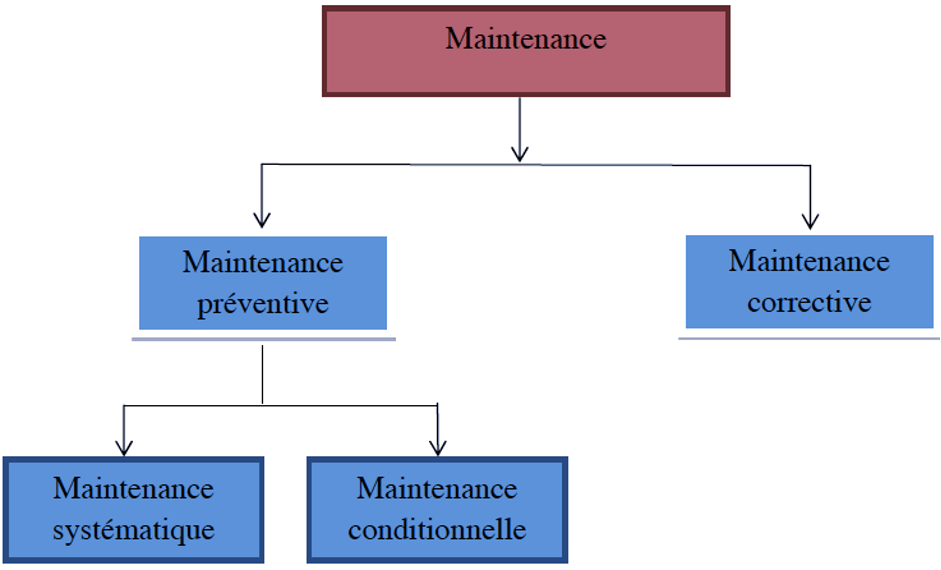
\includegraphics{images/mait_orga.png}
    \caption{Types de maintenances}
\end{figure}

\section{Les objectives de la maintenance}
Les objectifs de la fonction maintenance sont :\\
•	Contribuer à assurer la production prévue.\\
•	Veiller au respect des délais.\\
•	Contribuer à maintenir la qualité du produit fabriqué.\\
•	Rechercher les coûts optimaux.\\
•	Préserver l’environnement de production.\\

Ces objectifs généraux assignés à la maintenance impliquent des missions multiples, d’où l’attribution de moyens importants : leur pleine rentabilisions amène très souvent la maintenance à assurer des missions qui, entre autres, peuvent dépasser le cadre strict de cette fonction.

\section{Pourquoi une maintenance informatisée}
L’inefficacité de la méthode papier, en raison de son incapacité à transmettre l’information en temps réel, 
a poussé les acteurs industriels à étudier de nouveaux concepts de gestion plus exacte et à intégrer 
l’informatique au sein des entreprises industrielles afin d’optimiser l’information.

Concrètement, la mise en place des systèmes de gestion de maintenance informatisée entraîne :\\
•	Une méthode plus écologique\\
•	La réduction du temps consacré à la maintenance préventive\\
•	La diminution des heures supplémentaires (pannes réparées en dehors des heures normales)\\
•	La diminution des pertes de productions dues aux pannes (manque à gagner)\\
•	La diminution du temps consacré à la gestion administrative du service maintenance\\
•	Prolongation de la durée de vie des équipements grâce à une maintenance préventive mieux gérée\\
\pagebreak